\documentclass[conference]{IEEEtran}
\IEEEoverridecommandlockouts
\usepackage{cite}
\usepackage{amsmath,amssymb}
\usepackage{graphicx}
\usepackage{booktabs}
\usepackage{xcolor}
\usepackage{tikz}
\usetikzlibrary{positioning,arrows.meta,fit,calc}
\usepackage{pgfplots}
\pgfplotsset{compat=1.18}
\usepackage{textcomp}
\usepackage[hidelinks]{hyperref}
\usepackage{url}

\newcommand{\todo}[1]{\textcolor{red}{[#1]}}

\begin{document}

\title{Fire-Fit: A Smart-TV Personal Trainer That Uses the Viewer's Phone as a Private Pose and Voice Sensor}

% TODO(author): replace with your name, department, institution and e-mail.
\author{\IEEEauthorblockN{\todo{Author Name}}
\IEEEauthorblockA{\todo{Department, Institution}\\
\todo{City, Country}\\
\todo{e-mail}}}

\maketitle

\begin{abstract}
Smart TVs are the largest screen in most homes and a natural place to exercise, but
they have no camera or microphone that apps can use, so TV workout apps cannot count
repetitions, check form or respond to the user. We present Fire-Fit, a personal
trainer for Amazon Fire TV and Vega OS in which the TV runs the session and the
viewer's own phone, opened from a QR code, acts only as its sensor. The phone runs
MediaPipe pose estimation in the browser, so video never leaves it; only rep events,
form cues and recognised voice commands are relayed to the TV. A large language model
(Amazon Nova~2 Lite on Amazon Bedrock) generates each workout as schema-validated
structured output. The core of the system is a rule-based rep counter for 19 exercise
families with a set of robustness mechanisms: 3D world landmarks, aspect-ratio
correction, frame and posture gating, side selection, a start-position rule, minimum
rep durations, alternation for bilateral moves and One~Euro smoothing. On a synthetic
benchmark of 246 sequences built from the app's 23 counted exercise animations under
six camera conditions, the full counter reaches a macro-averaged mean absolute error
(MAE) of 0.063 and an off-by-one accuracy (OBOA) of 92.1\% with no phantom reps on
distractor motion, against 0.212, 78.3\% and 6.3 phantom reps for a naive counter.
An ablation shows that 3D world landmarks matter most (frontal-view MAE 0.051 vs.\
0.778 without them). We release the benchmark and a protocol for a real-video study.
\end{abstract}

\begin{IEEEkeywords}
human pose estimation, repetition counting, smart TV, fitness, multi-device interaction, large language models
\end{IEEEkeywords}

%======================================================================
\section{Introduction}
Home workouts on a TV usually mean choosing from a library of fixed videos. Nobody
adjusts the session to the person, counts their reps or notices that a squat is too
shallow. Camera-based coaching exists on phones and laptops~\cite{chen2020posetrainer,fieraru2021aifit},
but the TV, the screen people actually exercise in front of, rarely has a camera, and
TV platforms such as Vega OS offer apps no audio-capture or speech-recognition API.

Fire-Fit addresses this with a split design: \emph{the TV runs the workout, the phone is
its eyes and ears}. The TV shows the session (an animated demonstration figure,
countdowns, form tips, calories), while a phone propped two to three metres away runs
pose estimation and speech recognition in its browser. Pairing is by QR code, with
nothing to install. The same counter runs directly in a laptop browser when a webcam
is present.

This paper makes four contributions:
\begin{enumerate}
\item A \textbf{phone-as-sensor architecture} for camera-less TVs that keeps video on
the phone and sends only discrete events (Section~\ref{sec:system}).
\item A \textbf{rule-based rep counter} for 19 exercise families with eight
switchable robustness mechanisms, small enough to run identically on the TV, phone and
laptop (Section~\ref{sec:counter}).
\item A \textbf{synthetic benchmark and ablation} that generates labelled pose
sequences from the app's own exercise animations under realistic camera degradations
(Section~\ref{sec:eval}).
\item An open \textbf{real-video evaluation protocol} and tooling (Section~\ref{sec:real}).
\end{enumerate}

%======================================================================
\section{Related Work}
\textbf{Pose estimation.} OpenPose~\cite{cao2021openpose} made multi-person 2D pose
estimation practical; BlazePose~\cite{bazarevsky2020blazepose}, distributed through
MediaPipe~\cite{lugaresi2019mediapipe}, runs on phones in real time and also estimates
metric 3D ``world'' landmarks. Fire-Fit uses the MediaPipe Pose Landmarker in the browser.

\textbf{Repetition counting.} Learned counters such as RepNet~\cite{dwibedi2020repnet}
and TransRAC~\cite{hu2022transrac} count repetitions of arbitrary actions from video;
earlier work counted live from motion periodicity~\cite{levy2015live}. These methods
are class-agnostic but heavy for a phone browser and do not explain \emph{why} a rep
did not count. GymCam~\cite{khurana2018gymcam} tracks exercises with a fixed camera in a
gym. Rule-based counters on pose keypoints, as in Pose Trainer~\cite{chen2020posetrainer},
are interpretable and cheap but fragile; this paper studies which mechanisms make such
a counter robust. We adopt RepNet's MAE and OBOA metrics.

\textbf{Form feedback.} AIFit~\cite{fieraru2021aifit} learns interpretable 3D feedback
models. Fire-Fit uses hand-written per-family checks (squat depth, hip sag, lockout)
because they can be explained in one spoken sentence.

%======================================================================
\section{System Design}\label{sec:system}

\begin{figure}[t]
\centering
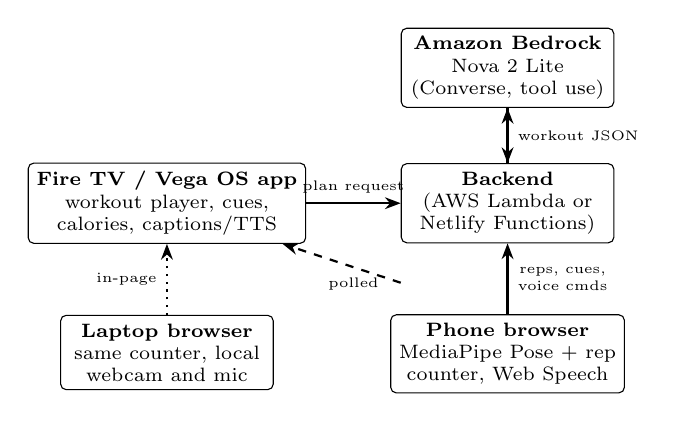
\begin{tikzpicture}[
  box/.style={draw, rounded corners=2pt, align=center, font=\scriptsize, minimum height=7mm, inner sep=3pt},
  arr/.style={-{Stealth[length=2mm]}, thick},
  lab/.style={font=\tiny, align=center}]
\node[box, minimum width=27mm] (tv) {\textbf{Fire TV / Vega OS app}\\workout player, cues,\\calories, captions/TTS};
\node[box, minimum width=27mm, right=12mm of tv] (be) {\textbf{Backend}\\(AWS Lambda or\\Netlify Functions)};
\node[box, minimum width=27mm, below=9mm of be] (ph) {\textbf{Phone browser}\\MediaPipe Pose + rep\\counter, Web Speech};
\node[box, minimum width=27mm, above=7mm of be] (br) {\textbf{Amazon Bedrock}\\Nova 2 Lite\\(Converse, tool use)};
\node[box, minimum width=27mm, below=9mm of tv] (lp) {\textbf{Laptop browser}\\same counter, local\\webcam and mic};
\draw[arr] (tv) -- node[lab, above]{plan request} (be);
\draw[arr] (be) -- node[lab, right]{workout JSON} (br);
\draw[arr] (br) -- (be);
\draw[arr] (ph) -- node[lab, right]{reps, cues,\\voice cmds} (be);
\draw[arr, dashed] (be.west |- ph.north) ++(0,4mm) -- node[lab, below, pos=0.4]{polled} ($(tv.south east)+(-3mm,0)$);
\draw[arr, dotted] (lp) -- node[lab, left]{in-page} (tv);
\end{tikzpicture}
\caption{Fire-Fit architecture. Video stays on the phone or laptop; only events reach the TV.}
\label{fig:arch}
\end{figure}

Fig.~\ref{fig:arch} shows the components.

\textbf{TV app.} One React Native codebase targets Vega OS and Fire OS (and the web).
Screens are laid out at $1920\times1080$ and every dimension is converted to device
units before rendering, so text stays sharp on 720p--4K panels, including Android TV
devices that report $960\times540$\,dp. The user drives everything with the remote's
D-pad or by voice. Each of the 32 moves has a hand-built animated stick figure; the same
animations drive the benchmark in Section~\ref{sec:eval}.

\textbf{Workout generation.} The user picks a goal, duration, level, equipment and
limits (e.g., ``knee friendly''). The backend calls Amazon Nova~2 Lite through the
Bedrock Converse API~\cite{awsconverse} with a forced \texttt{emit\_workout} tool whose
JSON schema describes warm-up, main and cool-down segments. Every field is validated
and clamped before the TV sees it, and a deterministic generator is used if the model
is unavailable, so the TV never dead-ends.

\textbf{Phone companion.} Scanning the TV's QR code opens a web page bound to a
four-digit session. The page runs the Pose Landmarker (full model, lite fallback) at
up to 30\,fps and the Web Speech API~\cite{webspeech}. It posts rep events, form cues and
parsed commands (\emph{start, wait, skip, rest, slower, faster, easier, end}) to the
session; the TV polls it and speaks the cue. Sessions are stored in DynamoDB on AWS or
in Netlify Blobs. A laptop with a webcam runs the same code inside the TV web app with
no pairing; the mode is detected automatically.

\textbf{Calories.} Energy is estimated from the Mifflin--St~Jeor resting metabolic
rate~\cite{mifflin1990} and each move's MET value~\cite{ainsworth2011compendium}:
$\dot{E} = \mathrm{MET}\cdot\mathrm{BMR}/86400$ kcal\,s$^{-1}$.

\textbf{Privacy.} No frame leaves the phone or laptop. The backend sees only rep
counts, short cue strings and command words; body data for calories stays on the TV.

%======================================================================
\begin{table*}[t]
\caption{MAE / OBOA by camera condition}
\label{tab:conditions}
\centering
\small
% generated by backend/eval/synthetic.ts
\begin{tabular}{lrrrrrr}
\toprule
 & Clean & Noise & Occlusion & Frontal & Portrait & Flicker\\
\midrule
Full system & 0.040 / 96\% & 0.144 / 83\% & 0.064 / 88\% & 0.051 / 94\% & 0.040 / 96\% & 0.040 / 96\%\\
Baseline (all off) & 0.004 / 100\% & 0.103 / 87\% & 0.034 / 94\% & 0.713 / 28\% & 0.105 / 91\% & 0.312 / 70\%\\
\bottomrule
\end{tabular}

\end{table*}

\section{Rep Counter}\label{sec:counter}

Each exercise maps to one of 23 \emph{families}, 19 of which count reps (squat, lunge, push-up, hinge,
curl, press, row, bridge, crunch, burpee, jumping jacks, high knees, climbers, skater,
boxing, circles, marching, band pull-apart, halo). A family defines a scalar metric per frame, usually a joint angle
(knee angle for squats, elbow angle for push-ups) or a normalised distance (feet width
over torso length for jacks), plus form checks.

\textbf{Hysteresis counting.} For a ``down'' movement with thresholds $\ell < h$, a rep
is counted when the metric goes below $\ell$ and then back above $h$ (e.g., squat knee
angle $\ell=130^\circ$, $h=160^\circ$). The extreme value of the rep feeds the form check.

\textbf{Robustness mechanisms.} Each can be disabled for ablation:
\begin{itemize}
\item \emph{3D world landmarks}: angles from metric 3D landmarks, so a squat seen from
the front still shows knee flexion.
\item \emph{Aspect correction}: without 3D data, image $x$ is scaled by the frame's aspect
ratio before computing angles (portrait phones).
\item \emph{Frame gating}: frames are ignored if a needed joint has visibility $<0.65$ or
jumps more than 0.6 torso lengths between frames (a guessed, occluded joint).
\item \emph{Posture gate}: each family has an expected torso posture (upright, squatting,
lying, prone); curls do not count as push-ups.
\item \emph{Sticky side}: in side view the more visible side is used and kept, so the
counter does not flip between left and right on flicker.
\item \emph{Start rule}: the counter arms only after the start position is seen, so
walking into frame mid-squat is not a rep.
\item \emph{Minimum duration}: a rep faster than a family-specific minimum (e.g., 500\,ms
for squats, 300\,ms for jacks) is rejected, and stage-based families must hold a stage
for 150\,ms.
\item \emph{Alternation}: alternating moves (marching, high knees, climbers) count a leg only after
the other side.
\end{itemize}
Landmarks are smoothed with a One~Euro filter~\cite{casiez2012oneeuro}. A half-finished
rep is dropped after 8\,s or when the person is lost from view.

The counter is about 700 lines of TypeScript with no dependencies. The same file runs on
the phone, laptop and TV; a test asserts the copies are identical. It costs about
30\,\textmu s per frame (filter and rules) in Node.js~22 on a 2.1\,GHz Xeon core,
negligible against the 33\,ms frame budget.

%======================================================================
\section{Synthetic Evaluation}\label{sec:eval}

\textbf{Benchmark.} Real labelled footage is expensive, so we first built a controlled
benchmark from the app's 23 counted exercise animations. Each animation is played for
six cycles at 30\,fps and converted to the 33 BlazePose landmarks, giving a known true
count (bilateral moves count each side). Six conditions model camera input:
\emph{clean}; \emph{noise} (Gaussian landmark noise, $\sigma=0.012$ of frame size);
\emph{occlusion} (12\% of frames have one limb joint displaced by up to 0.2 with low
visibility); \emph{frontal} (side-view moves rotated to face the camera, 18 exercises);
\emph{portrait} (aspect 0.75, no 3D data); and \emph{flicker} (far-side joints jitter and
alternate in visibility). Noise and occlusion use three seeds. We add 21 distractor
sequences with true count zero: 5\,Hz shaking in four exercises' poses, and the wrong
exercise (curls when push-ups are expected, marching for crunches, squats for bridges).
In total there are 246 sequences.

\textbf{Metrics.} Following RepNet~\cite{dwibedi2020repnet}, MAE $=\frac{1}{N}\sum
|\hat{c}-c|/c$ and OBOA is the share of sequences with $|\hat{c}-c|\le1$. Phantom reps
are the mean count on distractors. Averages are macro-averages over the six conditions.

\textbf{Configurations.} The full system; the full system minus each mechanism; minus the
One~Euro filter; and a baseline with everything off.

\begin{table}[t]
\caption{Ablation on the synthetic benchmark (macro-average over six conditions)}
\label{tab:ablation}
\centering
\small
% generated by backend/eval/synthetic.ts
\begin{tabular}{lrrr}
\toprule
Configuration & MAE $\downarrow$ & OBOA $\uparrow$ & Phantom $\downarrow$\\
\midrule
Full system & 0.063 & 92.1\% & 0.00\\
$-$\,3D world landmarks & 0.190 & 78.6\% & 0.00\\
$-$\,aspect correction & 0.085 & 89.9\% & 0.00\\
$-$\,frame gating & 0.063 & 92.1\% & 0.00\\
$-$\,posture gate & 0.063 & 92.1\% & 0.00\\
$-$\,sticky side & 0.111 & 87.7\% & 0.00\\
$-$\,start rule & 0.036 & 96.9\% & 0.00\\
$-$\,min. duration & 0.063 & 92.1\% & 5.00\\
$-$\,alternation & 0.063 & 92.1\% & 0.00\\
$-$\,One Euro filter & 0.065 & 91.3\% & 0.00\\
Baseline (all off) & 0.212 & 78.3\% & 6.33\\
\bottomrule
\end{tabular}

\end{table}


\begin{figure}[t]
\centering
\begin{tikzpicture}
\begin{axis}[
  ybar, width=\columnwidth, height=42mm, bar width=4pt,
  symbolic x coords={clean,noise,occlusion,frontal,portrait,flicker},
  xtick=data, x tick label style={font=\scriptsize},
  ylabel={MAE}, ylabel style={font=\scriptsize}, yticklabel style={font=\scriptsize},
  ymin=0, legend style={font=\tiny, at={(0.5,1.03)}, anchor=south, draw=none, legend columns=3},
  enlarge x limits=0.1]
\addplot table[x=cond, y=full, col sep=comma] {results/conditions.csv};
\addplot table[x=cond, y=noworld, col sep=comma] {results/conditions.csv};
\addplot table[x=cond, y=base, col sep=comma] {results/conditions.csv};
\legend{Full system, $-$ 3D world landmarks, Baseline}
\end{axis}
\end{tikzpicture}
\caption{MAE by condition (lower is better).}
\label{fig:conditions}
\end{figure}

\textbf{Results.} Tables~\ref{tab:conditions} and~\ref{tab:ablation} and Fig.~\ref{fig:conditions} show the
results. The full system reaches MAE 0.063 and OBOA 92.1\% with no phantom reps,
against 0.212, 78.3\% and 6.3 phantom reps for the baseline.

\emph{3D world landmarks} matter most: without them frontal-view MAE rises from 0.051
to 0.778, because knee and hip flexion is nearly invisible in a 2D frontal projection.
\emph{Sticky side} prevents the flicker failure (MAE 0.040 vs.\ 0.330), \emph{aspect
correction} the portrait failure (0.040 vs.\ 0.170), and \emph{minimum duration}
removes all 10 phantom reps per shaking sequence.

Three findings were less flattering, and we report them as found. First, the
\emph{start rule} costs accuracy here (MAE 0.036 without it): seven animations begin
mid-rep, and the rule deliberately discards that first partial rep. In real use this
is the intended behaviour, but the benchmark penalises it. Second, under \emph{noise}
the full system is worse than the baseline (0.144 vs.\ 0.103): smoothing and gating
trade lost reps for zero false positives. Small-amplitude moves suffer most; dumbbell
and kettlebell halos lose every rep at $\sigma=0.012$. Third, removing frame gating,
the posture gate or alternation alone changes nothing on this benchmark, although the
baseline counts 2.7 phantom reps on wrong-exercise sequences: these protections
overlap, so only removing several exposes the failure. Real footage, with genuinely
occluded joints, is needed to separate them.

\textbf{Tuning.} An earlier filter setting ($f_{c,\min}=1.2$\,Hz, $\beta=0.5$) over-smoothed
fast moves: with it, the full system missed every high-knee and mountain-climber rep
and reached only MAE 0.183 (OBOA 82.7\%). Raising $\beta$ to 20 and $f_{c,\min}$ to
1.5\,Hz restored them; adding the 150\,ms stage hold for jacks then removed the phantom
reps that faster filtering let through. The benchmark exposed both problems before users did.

%======================================================================
\section{Real-Video Study}\label{sec:real}

Synthetic sequences come from the same animations that the thresholds were designed
against, so they measure robustness to degradations, not accuracy on people. We
therefore define a real-video protocol and release the tooling: participants record
8--15 reps of eight exercises from side and front views with a phone (portrait, 2--3\,m
away) and a laptop webcam, plus distractor clips. Two annotators count each clip
independently and resolve disagreements together. Landmarks are extracted offline with
the same Pose Landmarker model, and the same ablations are scored.

\IfFileExists{results/real_ablation.tex}{%
\begin{table}[t]
\caption{Ablation on real videos}
\label{tab:real}
\centering
\small
\input{results/real_ablation.tex}
\end{table}
Table~\ref{tab:real} shows the results. \todo{Describe the dataset (people, clips, exercises, inter-rater agreement) and discuss the results.}
}{%
\todo{Real-video results pending: record the clips (backend/eval/real/README.md), run the scorer, and rebuild; the table is inserted automatically.}
}

%======================================================================
\section{Limitations}
The synthetic benchmark shares its source with the counter's design, and its
degradations are simplified models of real camera error. The counter handles one person
and 19 counted families; new exercises need new rules, unlike class-agnostic counters such as
RepNet~\cite{dwibedi2020repnet}. Form checks are heuristics and have not been validated
against expert ratings. Calorie estimates use population equations and are approximate.

%======================================================================
\section{Conclusion}
Fire-Fit shows that a camera-less TV can still watch a workout by borrowing the viewer's
phone, without sending video anywhere. A small, interpretable counter can be made
robust with a handful of mechanisms, chiefly 3D world landmarks, and a synthetic
benchmark built from the app's own animations is a cheap way to find regressions
before users do. Future work is the real-video study, learned per-family thresholds,
and multi-person tracking.

\section*{Code and Data Availability}
\todo{Add repository URL.} The benchmark is reproduced with
\texttt{npx tsx eval/synthetic.ts}; the real-video tooling is in \texttt{eval/real/}.

\section*{Acknowledgment}
In line with IEEE policy on AI-generated content, we disclose that an AI assistant
(Anthropic's Claude) was used to help write the application code, the evaluation
scripts and a draft of this paper. All results come from running the released code;
the author reviewed and is responsible for all content. \todo{Edit to reflect exactly how you used AI tools.}

\bibliographystyle{IEEEtran}
\bibliography{refs}

\end{document}
